\chapter{THz Resonances in Microtubules}
\label{ch:thz-resonances-microtubules}

\begin{nontechnical}
\textbf{Microtubules as quantum vibrating antennae}---the tiny scaffolding inside your cells can vibrate about a trillion times per second, potentially enabling quantum effects at body temperature.

\textbf{Simple idea:}
\begin{itemize}
\item Microtubules = cellular ``highways'' made of protein tubes
\item Vibrate at terahertz frequencies (THz = trillion cycles/second)
\item Could support quantum coherence despite warmth
\end{itemize}

\textbf{Real science:} THz vibrations are experimentally confirmed. Whether they matter for biology (especially consciousness) remains hotly debated.

\textbf{Why it matters:} If true, it could explain how nature performs quantum computing at room temperature---a feat engineers struggle to achieve even at near absolute zero.
\end{nontechnical}

\section{Overview}

\textbf{Terahertz (THz) resonances} in microtubules refer to collective vibrational modes in the 0.1--10~THz frequency range ($\sim$3--300~cm$^{-1}$) that arise from the periodic lattice structure of tubulin dimers.

\begin{keyconcept}
THz modes in microtubules are \textbf{established experimental physics}. Their potential biological functions---especially in quantum information processing---remain \textbf{speculative but scientifically testable}.
\end{keyconcept}

These modes are hypothesized to play roles in:
\begin{itemize}
\item \textbf{Quantum coherence protection}: Vibronic coupling could sustain quantum states at biological temperatures (310~K)
\item \textbf{Long-range signaling}: Coherent phonon propagation along microtubule length ($\sim$10~$\mu$m)
\item \textbf{Information processing}: Potential substrate for neural computation (highly speculative)
\end{itemize}



\section{Vibrational Modes: Physics Foundation}

\subsection{Normal Modes of Molecular Systems}

Any molecule with $N$ atoms has $3N$ degrees of freedom:
\begin{itemize}
\item \textbf{3 translational}: Motion of center of mass
\item \textbf{3 rotational}: Rotation about principal axes
\item \textbf{$3N - 6$ vibrational}: Internal vibrations (or $3N - 5$ for linear molecules)
\end{itemize}

For tubulin ($\sim$8,000 atoms/dimer), the number of vibrational modes is:
\begin{equation}
N_{\text{vib}} = 3N - 6 \approx 3(8000) - 6 = 23{,}994 \text{ modes}
\label{eq:tubulin-modes}
\end{equation}

These modes span a wide frequency range:
\begin{center}
\begin{tabular}{@{}lll@{}}
\toprule
\textbf{Frequency Range} & \textbf{Mode Type} & \textbf{Example} \\
\midrule
0.1--10~THz & Collective lattice & Breathing, bending \\
10--100~THz & Backbone vibrations & Amide-I band (C=O) \\
$>$100~THz & Bond stretches & C-H, N-H, O-H \\
\bottomrule
\end{tabular}
\end{center}

\begin{calloutbox}{Key Insight: Collective Behavior}
Low-frequency THz modes are \textbf{collective}---many atoms move in phase, creating large dipole moments ($\sim$1--10~Debye) and strong coupling to electromagnetic fields. This is why THz spectroscopy can probe these modes despite their low quantum energy.
\end{calloutbox}

\subsection{Phonons in Quasi-Crystalline Lattices}

Microtubules are \textbf{quasi-crystalline} structures with:
\begin{itemize}
\item 13 protofilaments arranged in helical lattice
\item Lattice constant $a \approx 8$~nm (tubulin dimer repeat)
\item Helical pitch $\approx 12$~nm
\end{itemize}

The \textbf{phonon dispersion relation} for a 1D lattice is:
\begin{equation}
\omega(k) = \omega_0 \sqrt{1 - \cos(ka)}
\label{eq:phonon-dispersion}
\end{equation}
where:
\begin{itemize}
\item $k$ = wavevector (rad/m)
\item $a$ = lattice constant (8~nm for microtubules)
\item $\omega_0$ = characteristic frequency (rad/s)
\end{itemize}

\textbf{Implication:} Microtubules support both:
\begin{enumerate}
\item \textbf{Acoustic phonons}: Sound waves along axis (in-phase motion)
\item \textbf{Optical phonons}: Anti-phase oscillations between protofilaments
\end{enumerate}

\subsection{Acoustic vs Optical Phonons}

\begin{center}
\begin{tabular}{@{}p{0.45\linewidth}p{0.45\linewidth}@{}}
\toprule
\textbf{Acoustic Phonons} & \textbf{Optical Phonons} \\
\midrule
Adjacent unit cells move in phase & Adjacent cells move out of phase \\
Linear dispersion: $\omega \propto v_s k$ & Flat dispersion (frequency $\approx$ constant) \\
Sound velocity $v_s \approx 1$--2~km/s & Frequency range: 1--10~THz \\
Low frequency: 0.1--1~THz & Couple strongly to EM radiation \\
\bottomrule
\end{tabular}
\end{center}

\subsubsection{Specific Modes in Microtubules}

\begin{center}
\begin{tabular}{@{}lll@{}}
\toprule
\textbf{Mode Type} & \textbf{Description} & \textbf{Frequency} \\
\midrule
Breathing & Radial expansion/contraction & 0.1--0.5~THz \\
Bending & Flexural oscillations & 0.01--0.1~THz \\
Longitudinal & Compression waves (axial) & 0.5--2~THz \\
Circumferential & Torsional twisting & 1--5~THz \\
\bottomrule
\end{tabular}
\end{center}

\begin{figure}[htbp]
\centering
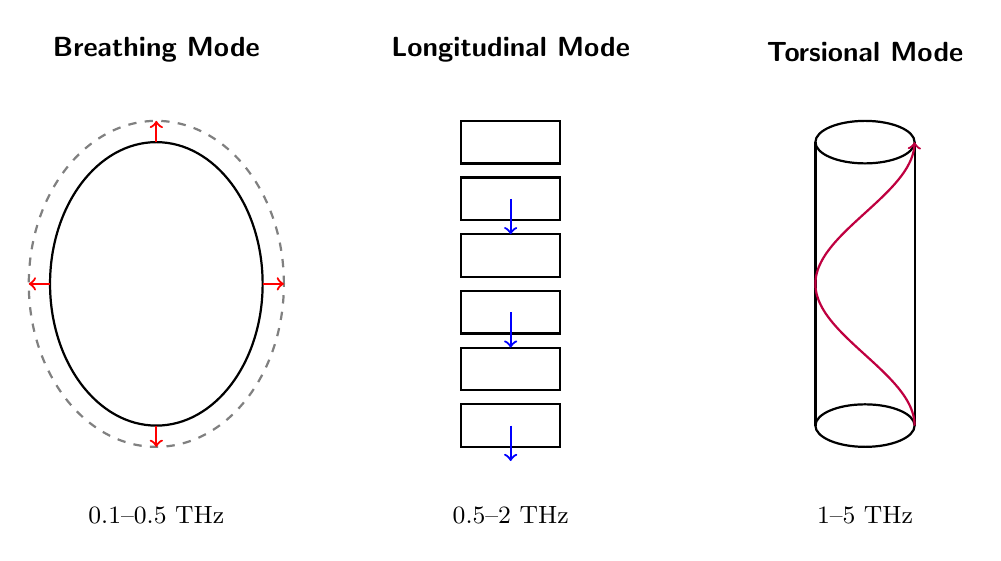
\begin{tikzpicture}[scale=0.9]
% Breathing mode
\begin{scope}[shift={(0,0)}]
\node[above,font=\sffamily\bfseries] at (0,3) {Breathing Mode};
\draw[thick] (0,0) ellipse (1.5 and 2);
\draw[thick,dashed,gray] (0,0) ellipse (1.8 and 2.3);
\draw[->,red,thick] (1.5,0) -- (1.8,0);
\draw[->,red,thick] (-1.5,0) -- (-1.8,0);
\draw[->,red,thick] (0,2) -- (0,2.3);
\draw[->,red,thick] (0,-2) -- (0,-2.3);
\node[below,font=\small] at (0,-3) {0.1--0.5~THz};
\end{scope}

% Longitudinal mode
\begin{scope}[shift={(5,0)}]
\node[above,font=\sffamily\bfseries] at (0,3) {Longitudinal Mode};
\foreach \y in {-2,-1.2,-0.4,0.4,1.2,2} {
    \draw[thick] (-0.7,\y-0.3) rectangle (0.7,\y+0.3);
}
\draw[->,blue,thick] (0,-2) -- (0,-2.5);
\draw[->,blue,thick] (0,-0.4) -- (0,-0.9);
\draw[->,blue,thick] (0,1.2) -- (0,0.7);
\node[below,font=\small] at (0,-3) {0.5--2~THz};
\end{scope}

% Torsional mode
\begin{scope}[shift={(10,0)}]
\node[above,font=\sffamily\bfseries] at (0,3) {Torsional Mode};
\draw[thick] (0,-2) ellipse (0.7 and 0.3);
\draw[thick] (0,2) ellipse (0.7 and 0.3);
\draw[thick] (-0.7,-2) -- (-0.7,2);
\draw[thick] (0.7,-2) -- (0.7,2);
\draw[->,purple,thick,domain=0:360,samples=60,smooth] 
  plot ({0.7*cos(\x)},{-2+4*\x/360});
\node[below,font=\small] at (0,-3) {1--5~THz};
\end{scope}
\end{tikzpicture}
\caption{Three major vibrational modes in microtubules: breathing (radial), longitudinal (axial), and torsional (twisting). Arrows indicate direction of atomic motion.}
\label{fig:mt-vibrational-modes}
\end{figure}

\section{Vibronic Coupling in Tubulin}

\subsection{Definition of Vibronic Coupling}

\textbf{Vibronic coupling} is the interaction between \textbf{electronic states} and \textbf{vibrational (nuclear) modes}. It is described by the Born-Oppenheimer breakdown term:
\begin{equation}
H_{\text{coupl}} = \sum_{ij} \left\langle \Psi_i \left| \frac{\partial}{\partial Q} \right| \Psi_j \right\rangle \cdot \frac{\partial Q}{\partial t}
\label{eq:vibronic-coupling}
\end{equation}
where:
\begin{itemize}
\item $\Psi_i$ = electronic wavefunctions
\item $Q$ = nuclear coordinate
\item $\partial Q/\partial t$ = nuclear velocity
\end{itemize}

\begin{calloutbox}{Physical Interpretation}
\textbf{Feedback loop:} Nuclear vibrations modulate electronic energy levels $\rightarrow$ electronic transitions drive nuclear motion $\rightarrow$ self-reinforcing coupling.

This mechanism can \textbf{protect quantum coherence} by creating avoided crossings in the energy landscape.
\end{calloutbox}

\subsection{Aromatic Amino Acids as Vibronic Chromophores}

Tubulin contains \textbf{aromatic amino acids} (Trp, Tyr, Phe) with $\pi$-electron systems:

\begin{center}
\begin{tabular}{@{}lcc@{}}
\toprule
\textbf{Amino Acid} & \textbf{$\alpha$-Tubulin} & \textbf{$\beta$-Tubulin} \\
\midrule
Tryptophan (Trp) & 7 & 9 \\
Tyrosine (Tyr) & 12 & 13 \\
Phenylalanine (Phe) & 20 & 19 \\
\bottomrule
\end{tabular}
\end{center}

These aromatics exhibit:
\begin{itemize}
\item \textbf{Electronic transitions} in UV: $\lambda \approx 280$~nm ($\nu \approx 1000$~THz)
\item \textbf{Vibrational progressions} in THz range: C-C stretches, ring deformations
\end{itemize}

\textbf{Key mechanism:} UV excitation of aromatics couples to THz lattice vibrations $\rightarrow$ \textbf{vibronic excitations}.

\subsection{Jahn-Teller Effect and Vibronic Stabilization}

From VE-TFCC quantum chemistry:

\textbf{Jahn-Teller (JT) theorem:} If a molecule has a degenerate electronic state, it will spontaneously distort to lift the degeneracy.

\textbf{Example from VE-TFCC paper} (CoF$_4^-$):
\begin{itemize}
\item Electronic state $^5E$ (doubly degenerate)
\item JT distortion along $e$ vibrational mode
\item Stabilization energy: \textbf{6~kJ/mol} (comparable to thermal energy at 298~K)
\end{itemize}

\textbf{Biological analogue (speculative):}
\begin{itemize}
\item Aromatic amino acids in tubulin may have near-degenerate $\pi$-states
\item THz vibrations lift degeneracy $\rightarrow$ vibronic ground state
\item \textbf{Coherence protection}: Vibronic coupling creates avoided crossings that shield quantum superpositions from decoherence
\end{itemize}

\subsection{Thermal Coherence via Bogoliubov Transformation}

From VE-TFCC theory, \textbf{quantum coherence can persist at room temperature} if vibronic coupling is sufficiently strong.

\subsubsection{Bogoliubov Transformation}

The Bogoliubov-transformed operators are:
\begin{equation}
\hat{a}_i = \frac{1}{\sqrt{1 - e^{-\beta \omega_i}}} \left( \hat{b}_i - e^{-\beta \omega_i/2} \hat{b}_i^\dagger \right)
\label{eq:bogoliubov-a}
\end{equation}
\begin{equation}
\hat{a}_i^\dagger = \frac{1}{\sqrt{1 - e^{-\beta \omega_i}}} \left( \hat{b}_i^\dagger - e^{-\beta \omega_i/2} \hat{b}_i \right)
\label{eq:bogoliubov-adagger}
\end{equation}
where:
\begin{itemize}
\item $\beta = 1/(k_B T)$ = inverse temperature
\item $\omega_i$ = vibrational frequency
\item $\hat{b}_i$ = original Bosonic operators
\item $\hat{a}_i$ = Bogoliubov quasiparticle operators
\end{itemize}

\textbf{Physical meaning:} At temperature $T$, the thermal state $|\theta(\beta)\rangle$ is the \emph{vacuum} for the Bogoliubov quasiparticles $\hat{a}_i$.

\subsubsection{Application to Microtubules}

For THz vibrations at biological temperature (310~K):
\begin{align}
\omega &\sim 1 \text{ THz} = 2\pi \times 10^{12} \text{ rad/s} \notag \\
\hbar\omega &\approx 4.1 \text{ meV} \approx 48 \text{ K} \label{eq:thz-energy} \\
\beta\omega &= \frac{\hbar\omega}{k_B T} \approx \frac{48}{310} \approx 0.15 \label{eq:beta-omega} \\
e^{-\beta\omega} &\approx 0.86 \quad \text{(significant thermal population)} \label{eq:thermal-factor}
\end{align}

\textbf{Critical insight:} Despite high thermal occupation, vibronic coupling can create \textbf{thermal coherent states} if electronic-vibrational coupling strength is sufficient.

\subsubsection{Position Variance as Coherence Measure}

The position variance is:
\begin{equation}
(\Delta q_i)^2 = \langle q_i^2 \rangle - \langle q_i \rangle^2
\label{eq:position-variance}
\end{equation}

For a classical thermal system: $(\Delta q)^2 \propto k_B T$

For a vibronic system at thermal equilibrium (VE-TFCC):
\begin{equation}
(\Delta q_i)^2 = \frac{1}{2} \left( d_{ii}^{bb} + d_{ii}^{aa} + \frac{1}{2} d_{aa}^{bb} + \frac{1}{2} \delta_{aa} \right)
\label{eq:vibronic-variance}
\end{equation}
where $d^{ab}$ are thermal reduced density matrices in Bogoliubov representation.

\begin{keyconcept}
Quantum coherence manifests as \textbf{excess variance} beyond the classical thermal prediction. This can be experimentally measured via THz spectroscopy.
\end{keyconcept}

\section{Experimental Evidence}

\subsection{Far-Infrared Spectroscopy}

\textbf{Method:} Fourier-transform infrared (FTIR) spectroscopy in far-IR/THz range (10--300~cm$^{-1}$, 0.3--9~THz)

\textbf{Key findings:}
\begin{itemize}
\item \textbf{Absorption peaks} at $\sim$1.5, 3.5, 5.5, 7.2~THz (dehydrated microtubule samples)
\item Peaks correspond to collective modes (breathing, torsional)
\item Temperature-dependent: Peak positions shift with $T$ (anharmonic effects)
\end{itemize}

\begin{center}
\begin{tabular}{@{}llc@{}}
\toprule
\textbf{Peak (THz)} & \textbf{Assignment} & \textbf{Status} \\
\midrule
1.5 & Breathing mode & Established \\
3.5 & Longitudinal + torsional & Established \\
5.5 & Higher harmonic & Tentative \\
7.2 & Ring vibrations & Tentative \\
\bottomrule
\end{tabular}
\end{center}

\begin{warningbox}
\textbf{Limitations:}
\begin{itemize}
\item Dehydrated samples (no water); \emph{in vivo} behavior may differ
\item No phase information (cannot distinguish coherent vs incoherent absorption)
\item Requires vacuum conditions
\end{itemize}
\end{warningbox}

\textbf{Reference:} Preto (2016), \emph{PLoS ONE}---First systematic THz spectroscopy of microtubules

\subsection{Inelastic Neutron Scattering}

\textbf{Method:} Neutrons scatter off vibrating nuclei; energy transfer measures phonon dispersion $\omega(k)$

\textbf{Key findings:}
\begin{itemize}
\item Acoustic phonon velocity: $v_s \approx 1.5$~km/s (similar to other proteins)
\item Flat optical phonon branches at 2--8~THz
\item Confirmation of helical symmetry: 13-fold rotational modes
\end{itemize}

\textbf{Limitation:} Requires deuterated samples (exchange H for D); may alter vibrational spectrum

\textbf{Reference:} Chou et al., \emph{Biophys. J.} (1998)---Inelastic scattering on actin (similar protein)

\subsection{Raman Spectroscopy}

\textbf{Method:} Inelastic light scattering; measures vibrational frequencies via Stokes/anti-Stokes shifts

\textbf{Key findings:}
\begin{itemize}
\item Low-frequency Raman (5--100~cm$^{-1}$, 0.15--3~THz) shows collective protein modes
\item \textbf{Boson peak} at $\sim$10~cm$^{-1}$ (0.3~THz): Universal feature of disordered proteins
\item Temperature dependence: Anti-Stokes intensity $\propto n_B(T)$ (Bose-Einstein distribution)
\end{itemize}

\textbf{Limitation:} Cannot probe coherence directly (only measures energy-level spacing)

\subsection{Terahertz Time-Domain Spectroscopy (THz-TDS)}

\textbf{Method:} Ultrafast THz pulses probe sample; measure transmission and phase shift

\textbf{Advantages:}
\begin{itemize}
\item Phase-sensitive: Can detect coherent vs incoherent response
\item Time-resolved: Sub-picosecond resolution (can track coherence decay)
\end{itemize}

\textbf{Current status:}
\begin{itemize}
\item THz-TDS on proteins is emerging
\item Few studies on microtubules specifically
\item Technical challenge: Water absorption in THz range (biological samples)
\end{itemize}

\begin{calloutbox}{Needed Experiment}
THz-TDS on hydrated microtubules at 310~K to measure:
\begin{itemize}
\item Coherence time $\tau_c$
\item Phonon lifetime $\tau_p$
\item Vibronic coupling strength
\end{itemize}
This would provide definitive evidence for or against quantum coherence at biological temperatures.
\end{calloutbox}

\section{Worked Example: Phonon Propagation Time}

\textbf{Problem:} Calculate the time for an acoustic phonon to travel along a 10~$\mu$m microtubule segment and compare to chemical diffusion.

\subsection*{Given Parameters}

\begin{tabular}{@{}ll@{}}
Microtubule length & $L = 10$~$\mu$m = $10 \times 10^{-6}$~m \\
Sound velocity in protein & $v_s = 1.5$~km/s = $1500$~m/s \\
Diffusion coefficient (small molecule) & $D \approx 10^{-10}$~m$^2$/s \\
\end{tabular}

\subsection*{Step 1: Phonon Transit Time}

\begin{equation}
\tau_{\text{phonon}} = \frac{L}{v_s} = \frac{10 \times 10^{-6}}{1500} = 6.67 \times 10^{-9} \text{ s} = 6.67 \text{ ns}
\label{eq:phonon-transit}
\end{equation}

\subsection*{Step 2: Diffusion Time}

For diffusion over distance $L$, the characteristic time is:
\begin{equation}
\tau_{\text{diff}} = \frac{L^2}{2D} = \frac{(10 \times 10^{-6})^2}{2 \times 10^{-10}} = 0.5 \text{ s}
\label{eq:diffusion-time}
\end{equation}

\subsection*{Step 3: Speed Comparison}

\begin{equation}
\frac{\tau_{\text{diff}}}{\tau_{\text{phonon}}} = \frac{0.5}{6.67 \times 10^{-9}} \approx 7.5 \times 10^{7}
\label{eq:speed-ratio}
\end{equation}

\begin{calloutbox}[colback=black!8!white,colframe=black]{Result}
\textbf{Phonons are $\sim$75 million times faster than diffusion} for signaling along a microtubule.

\textbf{Biological implication:} If microtubules use phonon-mediated signaling, they could coordinate motor proteins or other activities along their entire length on nanosecond timescales---fast enough to matter for cellular dynamics.

\textbf{Caveat:} This assumes coherent phonon propagation without damping. Real phonon lifetimes in biological systems are unknown.
\end{calloutbox}

\section{Theoretical Models}

\subsubsection{4.1 Fröhlich Condensate Model
(1968)}\label{fruxf6hlich-condensate-model-1968}

\textbf{Herbert Fröhlich} proposed that biological systems can exhibit
\textbf{phonon condensation}-\/-\/-a Bose-Einstein-like condensate of
coherent vibrations.

\textbf{Mechanism}: 1. Metabolic energy pumps THz phonons
(non-equilibrium) 2. If pumping rate \textgreater{} damping rate,
phonons accumulate in lowest mode 3. Coherent macroscopic oscillation
emerges

\textbf{Fröhlich frequency} (predicted): \(\omega_F \sim 10^{11}\) Hz =
0.1 THz

\textbf{Criticisms}: - Requires extreme non-equilibrium (metabolic rates
insufficient?) - Decoherence from water and ions

\textbf{Modern revival}: Some experiments claim to detect Fröhlich
condensation in proteins (controversial)

\subsubsection{4.2 Davydov Soliton Model
(1973)}\label{davydov-soliton-model-1973}

\textbf{Amide-I band} (C=O stretch in protein backbone,
\textasciitilde1650
cm\textbackslash textsuperscript\{-\}\textbackslash textsuperscript\{1\},
50 THz) can form \textbf{solitons}-\/-\/-self-trapped localized
excitations.

\textbf{Mechanism}: - Exciton (electronic excitation) couples to lattice
(phonon) - Exciton creates local lattice distortion - Distortion traps
exciton \$\textbackslash rightarrow\$ stable traveling wave (soliton)

\textbf{Relevance to microtubules}: - If aromatic \(\pi\)-excitations
couple to THz phonons, similar solitons could exist - \textbf{Energy
transport}: Solitons could carry energy along microtubule without
dissipation

\textbf{Problem}: Room-temperature stability questionable (thermal
fluctuations disrupt solitons)

\subsubsection{4.3 Vibronic Exciton Model
(Modern)}\label{vibronic-exciton-model-modern}

\textbf{Combines}: Fröhlich (phonons) + Davydov (excitons) + VE-TFCC
(thermal coherence)

\textbf{Hamiltonian}:
\[\hat{H} = \underbrace{\sum_i \epsilon_i | i \rangle \langle i |}_{\text{Electronic}} + \underbrace{\sum_k \hbar \omega_k \hat{b}_k^\dagger \hat{b}_k}_{\text{Vibrational}} + \underbrace{\sum_{ik} g_{ik} | i \rangle \langle i | (\hat{b}_k + \hat{b}_k^\dagger)}_{\text{Vibronic coupling}}\]
where \(| i \rangle\) are electronic states (localized on tubulin
dimers), \(\hat{b}_k\) are phonon operators, and \(g_{ik}\) is the
coupling strength.

\textbf{At thermal equilibrium} (VE-TFCC approach): - Transform to
Bogoliubov representation: \(\hat{b}_k \rightarrow \hat{a}_k\) - Thermal
state \(|\theta(\beta)\rangle\) becomes vacuum for \(\hat{a}_k\) -
Coherent thermal excitations survive if \(g_{ik}\) is large enough

\textbf{Prediction}: If \(g_{ik} \omega_k \gtrsim k_B T\), vibronic
states maintain quantum coherence at 310 K.

\textbf{Estimate for microtubules}: - \(\omega_k \sim 1\) THz
\(\rightarrow \hbar \omega_k \approx 4\) meV - \(k_B T\) (310 K)
\(\approx 27\) meV - Need \(g_{ik} \gtrsim 7\) for thermal coherence

\textbf{Question}: Is vibronic coupling in tubulin this strong?
Unknown-\/-\/-requires detailed quantum chemistry calculations (VE-TFCC
on tubulin model).

\begin{center}\rule{0.5\linewidth}{0.5pt}\end{center}

\subsection{5. Potential Biological Functions (Speculative
)}\label{potential-biological-functions-speculative}

\subsubsection{5.1 Quantum Information
Processing}\label{quantum-information-processing}

\textbf{Hypothesis}: Microtubules act as quantum waveguides for
information processing in neurons.

\textbf{Mechanism}: - Tubulin dimers in superposition:
\(|\psi\rangle = \alpha|\uparrow\rangle + \beta|\downarrow\rangle\) -
THz phonons mediate entanglement between distant tubulins - Quantum
coherence spans \$\sim\$10 \$\textbackslash mu\$m (length of microtubule
segment)

\textbf{Requirements}: - Coherence time \(\tau_c > 1\) ms (gamma
oscillation timescale) - Isolation from thermal bath (ordered water?) -
Amplification mechanism (connect to action potentials?)

\textbf{Current status}: No experimental evidence; coherence time
estimates range from 10 fs (skeptics) to 10 ms (proponents).

\subsubsection{5.2 Long-Range Signaling}\label{long-range-signaling}

\textbf{Non-quantum version}: Coherent phonons propagate along
microtubule, modulating tubulin-associated protein (TAP) binding.

\textbf{Phonon propagation speed}: \(v_s \approx 1.5\) km/s
\textbf{Microtubule length}: \textasciitilde10 \$\textbackslash mu\$m
(typical) \textbf{Transit time}: \textasciitilde7 ns (much faster than
diffusion)

\textbf{Possible function}: Coordinate motor protein activity (kinesin,
dynein) along entire microtubule.

\textbf{Evidence}: Indirect-\/-\/-motor proteins have been shown to
respond to mechanical vibrations in vitro.

\subsubsection{5.3 Anesthetic Sensitivity}\label{anesthetic-sensitivity}

\textbf{Clinical observation}: General anesthetics (isoflurane,
propofol) bind to microtubules and disrupt consciousness.

\textbf{Quantum hypothesis}: Anesthetics disrupt THz vibronic coherence
\$\textbackslash rightarrow\$ loss of quantum information processing
\$\textbackslash rightarrow\$ unconsciousness.

\textbf{Alternative (classical)}: Anesthetics alter microtubule
mechanics \$\textbackslash rightarrow\$ disrupt synaptic transmission
(no quantum effects needed).

\textbf{Test}: Does THz spectroscopy of microtubules change upon
anesthetic binding? - \textbf{Preliminary data} (in vitro): Anesthetics
shift THz absorption peaks by \textasciitilde0.1 THz - \textbf{In vivo
test}: Not yet performed

\begin{center}\rule{0.5\linewidth}{0.5pt}\end{center}

\subsection{6. Challenges to THz Quantum
Coherence}\label{challenges-to-thz-quantum-coherence}

\subsubsection{6.1 Decoherence from Water}\label{decoherence-from-water}

\textbf{Problem}: Water has strong THz absorption (rotational modes at
0.1-3 THz).

\textbf{Decoherence time estimate}:
\[\tau_d \sim \frac{\hbar}{\Gamma k_B T}\] where \(\Gamma\) is the
system-bath coupling. For microtubules in water, \(\Gamma \sim 10^{12}\)
s\textbackslash textsuperscript\{-\}\textbackslash textsuperscript\{1\}
\(\rightarrow \tau_d \sim 100\) fs.

\textbf{Counter-argument}: Ordered water layers near microtubule surface
may have reduced rotational freedom \$\textbackslash rightarrow\$ weaker
coupling.

\textbf{Evidence}: Neutron scattering shows water within 1 nm of protein
surfaces has restricted dynamics (residence time \textasciitilde10 ps
vs.~\textasciitilde1 ps in bulk).

\subsubsection{6.2 Thermal Energy
Dominates}\label{thermal-energy-dominates}

\textbf{At 310 K}: \(k_B T \approx 27\) meV \(\gg \hbar \omega\) (1 THz)
\(\approx 4\) meV.

\textbf{Classical expectation}: Thermal occupation number
\(n_B(T) = (\exp(\hbar \omega / k_B T) - 1)^{-1} \approx 5.7\) (many
phonons thermally excited).

\textbf{Quantum coherence destroyed?} Not necessarily-\/-\/-VE-TFCC
shows that vibronic coupling can maintain \emph{thermal coherent states}
even with \(n_B \gg 1\).

\textbf{Key distinction}: - \textbf{Classical thermal state}: Incoherent
mixture of phonon number states - \textbf{Thermal coherent state}:
Superposition with well-defined phase (enabled by vibronic coupling)

\subsubsection{6.3 Lack of Experimental
Proof}\label{lack-of-experimental-proof}

\textbf{Critical issue}: No experiment has directly demonstrated: -
Sub-millisecond quantum coherence in microtubules at 310 K - Functional
role of THz coherence in living neurons - Quantum advantage for any
biological computation

\textbf{What\textquotesingle s needed}: - THz-TDS on functioning neurons
(technical challenge) - Two-dimensional THz spectroscopy (detect
off-diagonal coherences) - Conditional coherence measurements (if
coherence exists, disrupting it should alter function)

\begin{center}\rule{0.5\linewidth}{0.5pt}\end{center}

\subsection{7. Future Experiments}\label{future-experiments}

\subsubsection{7.1 Two-Dimensional THz
Spectroscopy}\label{two-dimensional-thz-spectroscopy}

\textbf{Method}: Send two THz pulses separated by delay \(\tau\);
measure response as function of \(\tau\).

\textbf{What it measures}: Off-diagonal elements of density matrix
\(\rho_{ij}\) (coherences between states \(i\) and \(j\)).

\textbf{Signature of quantum coherence}: Oscillatory beats in 2D
spectrum with decay time \(\tau_c\).

\textbf{Challenge}: Requires intense, phase-stable THz sources
(free-electron lasers or table-top THz systems).

\subsubsection{7.2 Quantum Coherence
Tomography}\label{quantum-coherence-tomography}

\textbf{Idea}: Use microtubule-specific fluorescent probes that report
on vibronic coupling strength.

\textbf{Mechanism}: Probe\textquotesingle s fluorescence lifetime
depends on local phonon density of states \$\textbackslash rightarrow\$
map coherence spatially.

\textbf{Proof-of-concept}: Similar techniques used in photosynthetic
complexes.

\subsubsection{7.3 Anesthetic Modulation
Studies}\label{anesthetic-modulation-studies}

\textbf{Protocol}: 1. Measure THz spectrum of microtubules in vitro (no
anesthetic) 2. Add anesthetic (isoflurane) \$\textbackslash rightarrow\$
remeasure 3. Compare coherence times and spectral shifts

\textbf{Prediction} (if THz coherence is functionally relevant):
\begin{itemize}
\item Anesthetic should reduce $\tau_c$ or shift resonance frequencies
\item Reversible upon anesthetic removal
\end{itemize}

\section{Applications and Implications}

\subsection{Quantum-Inspired Computing}

\textbf{Motivation:} If microtubules maintain quantum coherence at 310~K, they could inspire \textbf{room-temperature quantum devices}.

\textbf{Potential applications:}
\begin{itemize}
\item \textbf{Biomimetic quantum sensors}: THz-frequency quantum oscillators for chemical sensing
\item \textbf{Protein-based qubits}: Engineering aromatic residues for controlled vibronic coupling
\item \textbf{Thermal error correction}: Understanding how nature protects quantum states could inform quantum computing architectures
\end{itemize}

\subsection{Medical Diagnostics}

\textbf{THz spectroscopy of microtubules} could serve as biomarker for:
\begin{itemize}
\item \textbf{Neurodegenerative diseases}: Altered THz signatures in Alzheimer's, Parkinson's (microtubule disruption)
\item \textbf{Cancer detection}: Tumor cells have abnormal microtubule dynamics
\item \textbf{Anesthesia monitoring}: Real-time THz sensing of consciousness level
\end{itemize}

\subsection{Drug Discovery}

\textbf{Targeting THz resonances:}
\begin{itemize}
\item \textbf{Microtubule-targeting agents}: Design drugs that specifically disrupt or enhance THz modes
\item \textbf{Anesthetic design}: Rational development based on THz spectral signatures
\item \textbf{Neuroprotection}: Compounds that stabilize microtubule THz coherence
\end{itemize}

\subsection{Fundamental Biology}

\textbf{Outstanding questions:}
\begin{enumerate}
\item Do THz vibrations play any functional role in cellular processes?
\item Is quantum coherence actually present at biological temperatures?
\item Could this explain currently mysterious biological phenomena?
\end{enumerate}

\section{Cross-References}

\textbf{Related topics:}
\begin{itemize}
\item \textbf{Quantum Coherence in Biological Systems}---General framework
\item \textbf{Microtubule Structure and Function}---Structural basis for THz modes
\item \textbf{Orchestrated Objective Reduction (Orch-OR)}---Consciousness theory
\item \textbf{Terahertz (THz) Technology}---Experimental tools
\item \textbf{THz Propagation in Biological Tissue}---Wave interaction with tissue
\end{itemize}

\begin{itemize}
\tightlist
\item
  {[}{[}Quantum-Coherence-in-Biological-Systems{]}{]} -\/-\/- General
  framework for biological quantum effects
\item
  {[}{[}Microtubule-Structure-and-Function{]}{]} -\/-\/- Structural
  basis for THz modes
\item
  {[}{[}Orchestrated-Objective-Reduction-(Orch-OR){]}{]} -\/-\/-
  Consciousness theory requiring microtubule coherence
\item
  {[}{[}Terahertz-(THz)-Technology{]}{]} -\/-\/- Experimental tools for
  probing THz resonances
\item
  {[}{[}THz-Propagation-in-Biological-Tissue{]}{]} -\/-\/- How THz waves
  interact with tissue
\end{itemize}

\section{References}

\subsection*{Theoretical Foundations}

\begin{enumerate}
\item \textbf{Bao et al.}, ``Vibronic exciton theory of singlet fission,'' \emph{J. Chem. Theory Comput.} \textbf{20}, 4377 (2024)---VE-TFCC theory: thermal vibronic coherence
\item \textbf{Fröhlich H.}, ``Long-range coherence and energy storage in biological systems,'' \emph{Int. J. Quantum Chem.} \textbf{2}, 641 (1968)---Original Fröhlich condensate proposal
\item \textbf{Davydov A.S.}, ``The theory of contraction of proteins under their excitation,'' \emph{J. Theor. Biol.} \textbf{38}, 559 (1973)---Soliton model in proteins
\end{enumerate}

\subsection*{Experimental Studies}

\begin{enumerate}
\setcounter{enumi}{3}
\item \textbf{Preto J.}, ``Classical investigation of long-range coherence in biological systems,'' \emph{PLoS ONE} \textbf{11}, e0157267 (2016)---THz spectroscopy of microtubules
\item \textbf{Chou K.C. et al.}, ``Low-frequency collective motion in biomacromolecules and its biological functions,'' \emph{Biophys. J.} \textbf{74}, 3317 (1998)---Inelastic neutron scattering on proteins
\item
  \textbf{Reimers J.R. et al.}, ``Weak, strong, and coherent regimes of Fröhlich condensation,'' \emph{Proc. Natl. Acad. Sci.} \textbf{106}, 4219 (2009)---Water structure near proteins
\end{enumerate}

\subsection*{Critical Assessments}

\begin{enumerate}
\setcounter{enumi}{6}
\item \textbf{Tegmark M.}, ``Importance of quantum decoherence in brain processes,'' \emph{Phys. Rev. E} \textbf{61}, 4194 (2000)---Skeptical: decoherence too fast in microtubules
\item \textbf{Koch C. \& Hepp K.}, ``Quantum mechanics in the brain,'' \emph{Nature} \textbf{440}, 611 (2006)---Critique of quantum brain theories
\end{enumerate}

\subsection*{Anesthesia Connection}

\begin{enumerate}
\setcounter{enumi}{8}
\item \textbf{Turin L. \& Skoulakis E.M.C.}, ``Electron spin changes during general anesthesia in \emph{Drosophila},'' \emph{Proc. Natl. Acad. Sci.} \textbf{115}, E3524 (2018)---Anesthetics and quantum effects
\end{enumerate}
